% copyright (c) 2018 Groupoid Infinity

\documentclass{article}
\usepackage[english,russian]{babel}
\usepackage{listings}
\usepackage{amsmath}
\usepackage{amssymb}
\usepackage{amsthm}
\usepackage{mathtools}
\usepackage{url}
\usepackage{tikz-cd}
\usepackage[utf8]{inputenc}

\theoremstyle{definition}
\newtheorem{theorem}{Теорема}
\newtheorem{definition}{Визначення}
\newtheorem{exercise}{Вправа}
\newtheorem{example}{Приклад}
\newcommand*{\incmap}{\hookrightarrow}
\newcommand*{\thead}[1]{\multicolumn{1}{c}{\bfseries #1}}
\lstset{basicstyle=\small,inputencoding=utf8}

\addto\captionsrussian{\renewcommand{\contentsname}{Зміст}}
\addto\captionsrussian{\def\refname{Список використаних джерел}}
\addto\captionsrussian{\renewcommand{\abstractname}{Аннотація}}


\begin{document}

\title{Issue IX: Quantum Interpreter}
\author{Максим Сохацький $^1$}
\date{ \small $^1$ Національний технічний університет України \\
       «Київський Політехнічний Інститут» ім. Ігора Сікорського \\
       29 жовтня 2018 }
\maketitle

\begin{abstract}
Ця робота є спробою огляду існуючих мов програмування для квантових обчислень,
їх теоретичних основ та особливостей.
Як приклад розглядається дискретне перетворення Фур'є,
яке в якості вправи імплементується на двох мовах програмування:
практичній, імперативній QCL від Бернхарда Омера\cite{Omer2003} та
теоретичній формальній, функціональній мові програмування, лямбда-численні
з лінійними функціями від Андре ван Тондера\cite{Tonder2004}. Як висновок
пропонуємо нарис своєї мови PLQ для квантових обчислень з залежними,
залежними-лінійними та квантовими типами.
\\
{\bf Ключові слова}: Теорія типів, квантові комп'ютери
\end{abstract}
\tableofcontents

\newpage

\section{Попередні відомості}

\subsection{Лінійна алгебра}
Нотація Дірака це компактний формалізм лінійної алгебри який будемо застосовувати
для визначень квантової механіки\footnote{І.О. Вакарчук. Квантова Механіка. 2012}.

\begin{table}[h]
\centering
  \caption{Нотація Дірака}
 \begin{tabular}{lll}
    \hline
       Нотація & Визначення \\
    \hline
       $|\psi\rangle$ & загальний кет-вектор, наприклад $(c_0,...,c_n)^T$ \\
       $\langle\psi|$ & дуальний бра-вектор, наприклад $(c_0^*,...,c_n^*)$ \\
       $|n\rangle$ & n-й базис вектор стандартного базису $N=(|0\rangle,...,|n\rangle)$\\
       $|\tilde{n}\rangle$ & n-й базис вектор альтернативного базису $\tilde{N}=(|\tilde{0}\rangle,...,|\tilde{n}\rangle)$ \\
       $\langle\phi|\psi\rangle$ & скалярний добуток \\
       $|i,j\rangle$ & тензорний добуток базисних векторів $|i\rangle$ та $|j\rangle$ \\
       $|\phi\rangle\otimes|\psi\rangle$ & тензорний добуток \\
    \hline
  \end{tabular}
\end{table}

\begin{definition} (Векторний простір). Множина V називається векторни мпростором над
скалярним полем F, тоді і тільки тоді, коли визначені операції $+ :V \times V \rightarrow V$ (сума векторів)
та $\cdot:F\times V\rightarrow V$ (добуток скаляра та вектора) з наступними властивостями:
i) $(V,+)$ утворюють комутативну групу;
ii) $\lambda |\psi\rangle = |\psi\rangle \lambda$;
iii) $\lambda(\mu|\psi\rangle) = (\lambda\mu)|\psi\rangle$;
iv) $(\lambda+\mu)|\psi\rangle = \lambda|\psi\rangle + \mu|\psi\rangle$;
v) $\lambda(|\psi\rangle+|\varphi\rangle) = \lambda|\psi\rangle + \lambda|\varphi\rangle$.
Далі будемо розглядати скалярне поле комплексних чисел $F=C$.
\end{definition}

\begin{definition} (Скалярний добуток).
Функція $\langle\cdot|\cdot\rangle:V\times V\rightarrow C$ називається скалярним
добутком, тоді і тільки тоді, коли:
i) $\langle\psi|(\lambda\varphi\rangle+\mu|\chi\rangle) = \lambda\langle\psi|\varphi\rangle+\mu\langle\psi|\varphi\rangle$;
ii) $\langle\psi|\varphi\rangle = \langle\varphi|\psi\rangle^*$;
iii) $0 < \langle\psi|\psi\rangle \in \mathbb{R}$.
Скалярний добуток визначає норму
$\parallel|\psi\rangle\parallel = \sqrt{\langle\psi|\psi\rangle} = \parallel\psi\parallel$.
\end{definition}

\begin{definition} (Повний векторний простір).
Нехай V векторний простір з нормою $\parallel\cdot\parallel$ та $|\psi_n\rangle \in V$
послідовність векторів.
i) $|\psi\rangle$ є послідовністю Коші ттт. $\forall\epsilon>0\exists N>0 : \forall n,m> N, \parallel |\psi_n\rangle - |\psi_{n+1}\rangle\parallel < \epsilon$.
ii) $|\psi\rangle$ сходиться ттт. $\forall\epsilon>0\exists N>0 : \forall n> N, \parallel |\psi_n\rangle - |\psi\rangle\parallel < \epsilon$.
Простір V повний ттт. кожна послідовність Коші сходиться.
\end{definition}

\begin{definition} (Гільбертів простір).
Повний векторний простір H зі скалярний добутком $\langle\cdot|\cdot\rangle$ та
відповідною нормою $\parallel\psi\parallel=\sqrt{\langle\psi|\psi\rangle}$ називається Гільбертовим.
\end{definition}

\begin{definition} (Лінійний оператор).
Нехай V -- векторний простір, а А -- функція $A : V \rightarrow V$. Тоді А
називається лінійним оператором ттт.
$$
A(\lambda|\psi\rangle + \mu|\varphi\rangle) = \lambda A |\psi\rangle + \mu A |\varphi\rangle
$$
В $C^n$ лінійний оператор є матрицею $m \times n$
з елементами $a_{i,j} = \langle i | A | j \rangle$, де $A = \Sigma_{i,j} a_{i,j} | i\rangle\langle j|$.
За визначенням лінійності оператор А можно записати через лінійну суму векторів базису B:
$$
A : |n\rangle \rightarrow \Sigma_k a_{kn}|k\rangle, \text{\ де\ } |k\rangle \in B.
$$
\end{definition}

\begin{definition} (Тензорний добуток гільбертових просторів).
Нехай $H_1$ та $H_2$ --- Гільбертові простори з базисами $B_1$ та $B_2$.
Тоді тензорний добуток
$$
H = H_1 \otimes H_2 = \{ \Sigma_{|i\rangle \in B_1} \Sigma{|j\rangle \in B_2} c_{ij}|i,j\rangle \| c_{ij} \in \mathbb{C} \}.
$$
також Гільбертів простір з базисом $B = B_1 \times B_2$ та скалярним добутком:
$$
\langle i,j | i',j' \rangle = \langle i | i' \rangle \langle j | j' \rangle  = \delta_{ii'}\delta{jj'}, \text{\ де\ } |i\rangle,|i'\rangle \in B_1, |j\rangle,|j'\rangle \in B_2.
$$
\end{definition}

\begin{definition} (Тензорний добуток лінійних операторів).
Нехай A та B лінійні оператори на Гільбертових протосторах $H_1$ та $H_2$, тоді
тензорний добуток
$$
A \otimes B = \Sigma_{i,j}\Sigma_{i',j'}|i,j\rangle\langle i|A|i'\rangle\langle j|B|j'\rangle\langle i',j'|
$$
лінійний оператор на на гільбертовому просторі $H_1\otimes H_2$.
\end{definition}

\begin{definition} (Комутатор та антикомутатор).
Нехай A та B лінійні оператори на гільбертовому просторі H.
Оператор $[A,B] = AB - BA$ називається комутатором,
а ${A,B} = AB + BA$ називається антикомутатором.
\end{definition}

\section{Інтерпретація квантової механіки}

В залежності від того як саме моделюються та конструюються
гільбертові простори та гамільтоніани, виникають різні теорії,
від нерятивістської квантової електродинаміки до квантової хронодинаміки яка
вводить поняття кварків та глюонів.

Теорія квантових обчислень --- це ще одна теорія поверх абстрактного квантового формалізму та
є інтерпретацією квантової механіки.
Однак це не фізична теорія в тому сенсі, що вона не описує природній процес,
а є ближчою до схемотехніки, з квабітами та квантовими вентилями, без визначення
як саме моделюється квантова система, вона може бути або фізичним об'єктом або симулятором.

Точно так як для апаратного забезпечення будуються мови порграмування та вищі мови програмування,
так само для квантових обчислень, квантових станів та квантових логічних елементів (вентилів),
існують свої мови програмування. У наступній секції дамо огляд існуючих мов та підходів до їх
побудови, а тут дамо основні принципи та компоненти архітекти квантових
обчислень, аби пояснити основні мовні елементи, та їх перетворення.

\newpage
\subsection{Пам'ять квантового комп'ютера}

\begin{definition} (Квантовий біт). Квантовий біт або квабіт визначається як квантова система,
стан якої може бути повністю виражений як суперпозиція (лінійна комбінація)
двох ортонормованих власних базових станів
позначених $|0\rangle$ та $|1\rangle$. Загальний стан $|\psi\rangle$ квабіта  тоді визначається
як $|\psi\rangle = \alpha |0\rangle + \beta |1\rangle, |\alpha|^2 + |\beta|^2 = 1$.
Значення квабіта описується спостереженням $N=|1\rangle\langle{1}|$. $\langle{N}\rangle$ дає
вірогідність знайти систему в стані $|1\rangle$, якщо над квабітом були проведені виміри.
Простір станів квабіта є гільбертовим простором $H=\mathbb{C}^2$.
Ортонормована система ${|0\rangle,|1\rangle}$ називається обчислювальним базисом.
\end{definition}

\begin{definition} (Сфера Блоха).
Загальний стан квабіта може бути виражений в полярних координатах $\theta$ та $\phi$:
$$
|\psi\rangle=cos\frac{\theta}{2}|0\rangle+e^{i\phi}sin\frac{\theta}{2}|1\rangle.
$$
Одиничний вектор стану $|\psi\rangle$ називається вектором Блоха $\tilde{r}_\psi$, та має
наступну властивість $\tilde{r}_\phi=-\tilde{r}_\xi \leftrightarrow \langle\phi|\xi\rangle = 0$.
\begin{figure}[h]
  \centerline{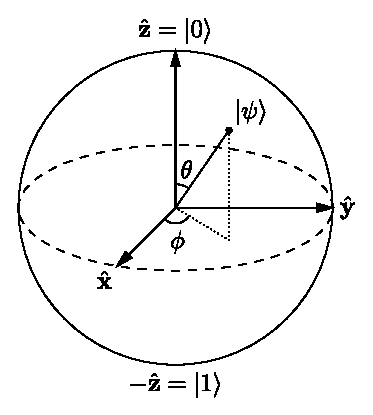
\includegraphics[scale=0.6]{bloch.eps}}
  \caption{Сфера Блоха як представлення квабіта $|\psi\rangle$}
\end{figure}
Оберти навколо осей X, Y та Z вектора Блоха тоді визначаються як оператори:
$$
X(\theta) = \begin{bmatrix}
cos\frac{\theta}{2} & -i sin\frac{\theta}{2} \\
-i sin\frac{\theta}{2} & cos\frac{\theta}{2} \\
\end{bmatrix},
Y(\theta) = \begin{bmatrix}
cos\frac{\theta}{2} & -sin\frac{\theta}{2} \\
sin\frac{\theta}{2} & cos\frac{\theta}{2} \\
\end{bmatrix},
Z(\theta) = \begin{bmatrix}
e^{-i\theta/2} & 0 \\
0 & e^{i\theta/2} \\
\end{bmatrix}
$$
\end{definition}

\begin{definition} (Квантова система).
\end{definition}

\begin{definition} (Еволюція системи).
Темпоральна еволюція стану системи описується рівнянням Шрьодінгера:
$$
i\hbar\frac{\delta}{\delta t}|\psi\rangle = H|\psi\rangle.
$$
де $\hbar \equiv 1.05457 \cdot 10^{-43}$ експериментальна константа Планка,
а $H$ --- фіксований самоспряжений оператор на гільбертовому просторі,
знаний як Гамільтоніан квантової системи. В квантовій фізиці нормують відносно
$\hbar$ тоді рівняння можна записани у безвимірній формі $i|\psi\rangle = H|\psi\rangle$.
Гамільтоніан H повністю визначає квантову систему.
Другий спосіб визначення, через унітарний оператор $U=e^{-iH}$.
Темпоральна еволюція замкненої квантової системи зі страну $|\psi\rangle$ та часу $t_1$
в стан $|\psi'\rangle$ та часу $t_2$ може бути описана унітарним оператором
$U = U (t_2 - t_1)$, таким, що $|\psi'\rangle = U |\psi\rangle$.
\end{definition}

\begin{definition} (Вимірювання).
Проективне вимірювання визначається як самоспряжений оператор M який називається
спостереженням зі спектральною композицією $M = \Sigma_m mP_m$, де $P_m$ проекція
на власний простір власного значення m. Власні значення m оператора M відповідаються
усім можливим результатам вимірювання. Вимірювання $|\psi\rangle$ дасть результат
m з вірогідністю $p(m) = \langle\psi|P_m|\psi\rangle$, таким чином через
скорочення $|\psi\rangle$ отримаємо новий стан системи $|\psi'\rangle = \frac{1}{\sqrt{p(m)}}P_m|\psi\rangle$.
Для стану квабіта, самоспряжений оператор N знаний як стандартне вимірювання.
$$
N = \begin{pmatrix} 0 & 0 \\ 0 & 1 \end{pmatrix} = 0 \cdot |0\rangle\langle 0| + 1 \cdot|1\rangle\langle1|.
$$
Біль загально для простору стану $H=C^n$ стандартне вимірювання визначається як $N=\Sigma_i i|i\rangle\langle i|$.
\end{definition}

\begin{definition} (Виважене середнє).
Виважене середнє $\langle M \rangle$ усіх можливих результатів вимірювання M називється
очікуваним значенням та визначається як
$$
\langle M\rangle = \Sigma_n p(m)m = \Sigma_m \langle\psi|m P_m|\psi\rangle = \langle \psi | M | \psi \rangle.
$$
\end{definition}

\subsection{Оператори обчислювального ядра}

\begin{definition} (Оператори Паулі).
Оператори Паулі пов'язані з довільним обертом вектора Блоха формулою:
$$
R_{\tilde{n}}(\theta) = e^{-\frac{i}{2}\theta\tilde{n}\cdot(x,y,z)} = cos\frac{\theta}{2}I - i sin\frac{\theta}{2} (n_x X + n_y Y + n_z Z)
$$
де X,Y,Z --- оператори:
$$
X=
\begin{bmatrix}
0 & 1 \\
1 & 0 \\
\end{bmatrix},
Y=
\begin{bmatrix}
0 & -i \\
i & 0 \\
\end{bmatrix},
Z=
\begin{bmatrix}
0 & -i \\
i & 0 \\
\end{bmatrix}
$$
\end{definition}

Найпростіший випадок унітарного перетворення це оператор який діє на одиничний квабіт.
Загальна форма 2-вимірної комплексної унітарної матриці $U \in SU(2)$ має вигляд:
$$
U = e^{i\varphi}\begin{pmatrix}
e^{\frac{i}{2}(-\alpha-\beta)}cos\frac{\theta}{2} & -e^{\frac{i}{2}(-\alpha+\beta)}sin\frac{\theta}{2} \\
e^{\frac{i}{2}(\alpha-\beta)}cos\frac{\theta}{2} & e^{\frac{i}{2}(\alpha+\beta)}sin\frac{\theta}{2} \\
\end{pmatrix}
$$

Нехай $U \in SU(2)$ має базисні вектори $|u\rangle$ та $|v\rangle$ та
власні значення $u$ та $v$. Тоді U можна виразити:
$$
U = u|u\rangle\langle u|+v|v\rangle\langle v| = e^{i\varphi}R_{\tilde{n}}(\delta),
$$
де $\delta$ --- фазова різниця між $u$ та $v$ --- пов'язана як $v = e^{i\delta}v$.

\begin{definition} (Оператор Адамара).
$$
H=\frac{1}{\sqrt{2}}
\begin{bmatrix}
1 & 1 \\
1 & -1 \\
\end{bmatrix}
$$
\end{definition}

\begin{definition} (Фазовий та $\pi/8$ оператори).
$$
S=
\begin{bmatrix}
1 & 0 \\
0 & i \\
\end{bmatrix},
R_3=
\begin{bmatrix}
1 & 0 \\
0 & e^{i\pi/4} \\
\end{bmatrix}
$$
\end{definition}

\begin{definition} (Контрольований вентиль).
Нехай U унітарний q-квабітний вентиль, контрольований U-венииль з n-контрольними бітами
тоді визначається як
$$
C^m[U] =
\begin{bmatrix}
I & \dots & 0 & 0 \\
\vdots & \ddots & 0 & 0 \\
0 & 0 & I & 0 \\
0 & 0 & 0 & U
\end{bmatrix}
$$
в просторі станів $B^{\otimes n+m}$.
\end{definition}

\begin{definition} (Контрольований НЕ вентиль).
$$
CNot : |x,y\rangle \rightarrow |x\otimes y,y\rangle
$$
$$
CNot=C[X]=
\begin{bmatrix}
I & 0 \\
0 & X \\
\end{bmatrix}
=
\begin{bmatrix}
1 & 0 & 0 & 0 \\
0 & 1 & 0 & 0 \\
0 & 0 & 0 & 1 \\
0 & 0 & 1 & 0 \\
\end{bmatrix}
$$
\end{definition}

\begin{definition} (Вентиль перестановки).
$$
Swap : |x,y\rangle \rightarrow |y,x\rangle
$$
\end{definition}

\begin{definition} (Контрольований фазовий вентиль).
$$
CPhase : |x,y\rangle \rightarrow i^{xy}|x,y\rangle
$$
\end{definition}

\begin{definition} (Вентиль Тофолі).
$$
CCNot : |x,y,z\rangle \rightarrow i^{xy}|x,y\rangle
$$
\end{definition}

\newpage
\section{Огляд існуючих мов}
З огляду на новизну предмету розроблено не так багато мов, усі що є можна розділіти
на імперативні (по духу своєї імплемантації) та функціональні (або побудовані на базі певного виду
лямбда числення). Ми наведемо приклади програм для обох підходів.
У якості порівняльної характеристики візьмемо алгоритм дискретного перетворення Фур'є.

\begin{figure}[h]
  \centerline{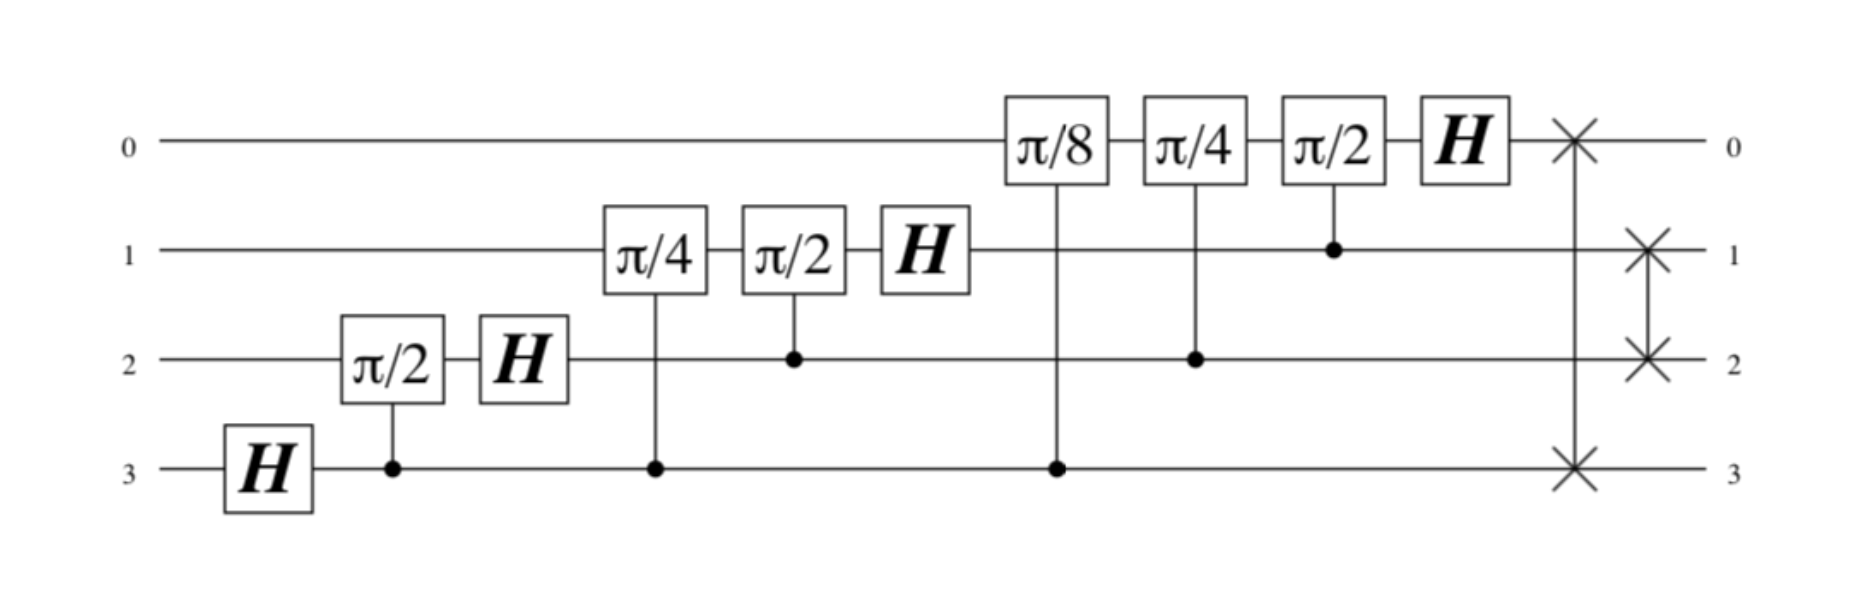
\includegraphics[scale=0.3]{fourier.png}}
  \caption{Графічне представлення квантової схеми вентилів дискретного перетворення Фур'є для 4-квабітного регістру}
\end{figure}

\newpage
\subsection{Імперативні мови програмування}
Станом на 2018 рік найбільш розробленою мовою, яка компілюється під Linux та Mac
є QLC від Бернхарда Омера
\footnote{Bernhard Ömer. Structured Quantum Programming. PhD. TU Vienna. 2003.
          \url{http://tph.tuwien.ac.at/~oemer/doc/structquprog.pdf}}.
До QLC можна відзначти наступні мови:
1) Q-gol від Грега Бейкера (1996)
   \footnote{Gregory David Baker.
             Qgol. A system for simulating quantum computations:
             Theory, Implementation and Insights. 1996. PhD. Macquarie University. \\
             \url{http://www.ifost.org.au/~gregb/q-gol/QgolThesis.pdf}};
2) qGCL від Паоло Зуліані (2000)\cite{Sanders2000};
3) Quantum C Language від Стефана Блаха (2002);
4) QPAlg від Марі Лолір та Філіпа Жорранда (2004)\cite{Lalire2004}, синтаксис та семантика цієї системи базується на численні процесів Мілнера CCS та формальній мові LOTOS;
5) CQP (Communication Quantum Processes) від Саймона Гея та Раджагопала Нагараджана (2004)\cite{Gay2005};
6) Q (DSL мова для С++) від Беттеллі, Каларко та Серафіні\cite{}.
7) LanQ від Гинека Млнаріка\cite{Mlnarik2007}.

\begin{definition} (Перестановка).
\begin{lstlisting}
cond qufunct Swap(qureg a,qureg b) {
  int i; if #a!=#b { exit "arguments must equal"; }
  for i=0 to #a-1 {
    CNot(b[i],a[i]);
    CNot(a[i],b[i]);
    CNot(b[i],a[i]); } }
\end{lstlisting}
\end{definition}

\begin{definition} (Зміна порядку квабітів).
\begin{lstlisting}
cond qufunct flip(qureg q) {
  int i; for i=0 to #q/2-1 { Swap(q[i],q[#q-i-1]); } }
\end{lstlisting}
\end{definition}

\begin{definition} (Дискретне перетворення Фур'є, Коперсміт).
\begin{lstlisting}
operator dft(qureg q) {
  const n=#q; int i; int j;
  for i=1 to n {
      for j=1 to i-1 { V(pi/2^(i-j),q[n-i] & q[n-j]); }
      H(q[n-i]); }
  flip(q); }
\end{lstlisting}
\end{definition}

\newpage
\subsection{Функціональні мови програмування}
Лямбда числення лежить в основі сучасних алгебраїчних систем та основ математики\cite{HoTT13},
воно може бути розглянуте не лише як мова програмування загального використання, але і
фреймворк для судження про обчислювальні властивості програм.

Таксономію лямбда числень, яку виконав Хенк Барендрегт та подав у вигляді лямбда кубу\cite{Henk93},
можна розширити квантовими мовними примітивами, вводити в вищі лямбда числення з
гомотопічними типами, або в системи доведення теорем з екстрактом або лише верифікацією.

З огляду на природу квантових обчислень необхідним компонентом квантового лямбда
числення є система лінійних типів, де за час існування змінної в області видимості
під час виконання дозволяється звертання до неї тільки один раз. Така система типів
уже використовується не тільки в еспериментальних верифікаторах але і в сучасних
системних мовах програмування (Rust), де завдяки верифікатору лініних типів
вдається обійтися без алгоритмів автоматичного вивільнення памяті під час
виконання програми (схема памяті повністю моделюється під час компіляції програми).

Серед робіт присвячених мовам на базі лямбда числень можна відзначити наступні:
1) Найбільш класичне нетипизоване лямбда числення Андре ван Тондера\cite{Tonder2004}.
   Тут подається доведення ізоморфізму машині Тюрінга, повнота та звучання системи,
   що є формальною перевагою перед імперативними мовами, такими як QCL;
2) Quipper від Гріна, Люмсдейна, Росса, Селінжера та Валірона \cite{Green2013}\cite{Green2013-2}.
   Це спроба вбудувати DSL для квантових обчислень в мову Haskell, симулятор
   мови побудований на генераторах групи Кліффорда, квантових операторах {X,Y,Z,H,S}.
3) Робота по лямбда численню від Аррігі та Довека\cite{Arrighi2004}.
4) QML для Haskell від Торстена Альтенкірха
   та Джонатана Граттажа\cite{Altenkirch2005}\cite{Altenkirch2007}\cite{Grattage2011}.

\newpage
\begin{definition} (Синтаксичне дерево O$_H$).
Синтаксичне дерево O$_H$ визначає лямбда числення з лінійними змінними
поєднане з класичним нетипизованим лямбда численням. Тобто O$_H$ є
найпростішим операційним квантовим лямбда численням для середовищ виконання.
\begin{lstlisting}[mathescape=true]
    c = $\textbf{0}$ | $\textbf{1}$ | $\textbf{H}$ | S | $R_3$ | $\textbf{CNot}$ | X | Y | Z | ...
    t = x | $\lambda$ x . t | $\textbf{let}$ x = t $\textbf{in}$ t | t t
          | (t,t) | t | c | ! t | $\lambda$ ! x . t
\end{lstlisting}
Тут даються примітиви лінійних типів, де доступ до змінної
можливий лише раз в обсласті визначення змінної. Для нелінійних або звичайних
лямбда функції даються примітиви позначені !. В переліку квантових примітивів
c даються:
i) ортонормований базис $|0\rangle$ та $|1\rangle$;
ii) H --- оператор Адамара;
iii) S --- фазовий вентиль;
iv) $R_3$ --- $\pi/8$ вентиль;
v) контрольований не вентиль CNot;
vi) вентилі Паулі X, Y та Z.
\end{definition}

\begin{definition} (Пара Айнштайна-Подольського-Розена).
\begin{equation}
\textbf{EPR} = \textbf{CNot}\ ((\textbf{H}\ \textbf{0}),\textbf{0})
\end{equation}
\end{definition}

\begin{definition} (Квантова телепортація).
\begin{multline}
\textbf{teleport}\ x = \textbf{let}\ (e_1,e_2)\ =\ \textbf{EPR in} \\
\textbf{let}\ (x',y') = \textbf{alice}\ (x,e_1)\ \textbf{in}\ \textbf{bob}\ (x',y',e_2) \\
\end{multline}
\begin{multline}
\textbf{alice}\ (x,e_1) = \textbf{let}\ (x',y') = \\
\textbf{CNot}\ (x,e_1)\ \textbf{in}\ ((\textbf{H}\ x'),y') \\
\textbf{bob}\ (x',y',e_2) = \textbf{let}\ (y'',e_2') = cX\ (y',e_2)\ \textbf{in} \\
\textbf{let}\ (x'',e_2'') = cZ\ (x',e_2')\ \textbf{in}\ (x'',y'',e_2'')
\end{multline}
\end{definition}

\begin{definition} (Дискретне перетворення Фур'є).
\begin{equation}
\textbf{fourier}\ list\ =\ \textbf{reverse fourier}'\ list
\end{equation}
\begin{multline}
\textbf{fourier}'\ list\ =
\ \textbf{case}\ list\ \textbf{of}
\begin{cases}
() \rightarrow () \\
h : t \rightarrow \textbf{let}\ h'\ :\ t' = \textbf{phases}\ (\textbf{H}\ h)\ t\ !2 \\
\textbf{in}\ h'\ :\ \textbf{fourier}'\ t'
\end{cases}
\end{multline}
\begin{multline}
\textbf{phases}\ target\ controls\ !n\ = \\
\textbf{case}\ control\ \textbf{of}
\begin{cases}
() \rightarrow target \\
control : t \rightarrow \textbf{let}\ (control',target') = \\
(cR\ !n)\ (control, target)\ \textbf{in} \\
\textbf{let}\ target'' : t' = \textbf{phases}\ target'\ t\ !(\textbf{succ}\ n)\ \textbf{in} \\
target '' : control' : t'
\end{cases}
\end{multline}
\end{definition}

\newpage
\section{Висновки}
Як видно для реалізації семантики мови програмування для квантових
комп'ютерів достатньо поєднаяти тензорне числення разом з $\pi$-численням процесів,
або лінійними типами. На сьогоднішній день (2018) серед імперативних мов програмування
найбільш завершена, повна та практична на думку автора є QLC від Бернхарда Омера, серед
мов для лямбда числень немає жодної достатньо зрілої імплементації.

\subsection{Мова PLQ}
Відкрите питання в теорії типів, імплементація та дизайн мови
з лінійними та залежними типами та квантовими примітивами.
Тому ми пропонуємо як висновок після огляду мов та їх синтаксисів свій синтаксис такої мови,
та показуємо з яких інгрідієнтів її можна побудувати.

Мову квантових обчислень O$_H$ можно розкласти до комбінації (прямої суми) трьох синтаксичних дерев:
  i) дерева O$_\lambda$ --- базового чистого лямбда числення з залежними типами (pure, імплементовану автором\cite{Tonpa18});
 ii) дерева O$_\pi$ --- числення з лінійними типами, або просто інший вид стрілок (linear);
iii) операторний базис квантового числення O$_Q$ з
     конструкторами X,Y,Z,S,H,R$_3$ та конструктором визначення квабіта (quantum).
Тоді формальний синтаксис мови для квантових комп'ютерів,
записаний на {\bf cubicaltt}\cite{Mortberg17} у вигляді індуктивного типу синтаксичного дерева,
буде виглядати так:
\begin{lstlisting}[mathescape=true]
${\bf data}$ pure (lang: U)
   = star (n: nat) | var (l: nat) | pi (l: nat) (f: lang)
   | lambda  (x: nat) (f: lang)   | app (f a: lang)
\end{lstlisting}
\begin{lstlisting}[mathescape=true]
${\bf data}$ linear (lang: U)
   = star (n: nat) | var (l: nat) | pi (l: nat) (f: lang)
   | lambda  (x: nat) (f: lang)   | app (f a: lang)
\end{lstlisting}
\begin{lstlisting}[mathescape=true]
${\bf data}$ quantum (lang: U)
   = register (n:nat) | i (n:nat) | 0 | 1 | H (l:lang) | S (:lang)
   | X (f:lang) | Y (f:lang) | Z (f:lang) | CNot (f a: lang)
\end{lstlisting}
Результуюча авторська мова (назвемо її PLQ) виражається
як взаяморекурсивна сума елментарних мовних синтаксисів.
\begin{lstlisting}[mathescape=true]
${\bf data}$ PLQ = Pure        (_: pure    PLQ)
         | Linear  (_: linear   PLQ)
         | Quantum (_: quantum PLQ)
\end{lstlisting}
З огляду на розмів реферату, семантику цієї мови наводити не будемо,
однак, очевидно, що мову Андре ван Тондера можна продовжиди до
PTS з лінійними типами в категоріях з сімейставами зі значеннями в симетричних моноїдальних категоріях,
як було показано Матейсом Вакаром\cite{Vakar2014}.
\newpage
\bibliographystyle{plain}
\bibliography{quantum}

\end{document}

